\documentclass[a4paper,12pt]{article}
\usepackage[T1]{fontenc}
\usepackage[utf8]{inputenc}
\usepackage{lmodern}
\usepackage[french]{babel}
\usepackage{url,csquotes}
\usepackage[hidelinks,hyperfootnotes=false]{hyperref}
\usepackage[titlepage]{polytechnique}
%\usepackage[titlepage,fancysections,pagenumber]{polytechnique}
\usepackage{float}
\usepackage{graphicx}
\usepackage{subfig}
\usepackage{tocloft}

\usepackage{tcolorbox}

\usepackage{titlesec}

% Define the font size for subsection headings
\titleformat{\subsubsection}
{\large\bfseries}{\thesubsubsection}{1em}{}

%\setcounter{tocdepth}{}
%\usepackage[charter]{mathdesign}

%\setcounter{secnumdepth}{0}


\title{Rapport de stage}
\subtitle{Stage linguistique à l'IFLS \\
Formation Préparatoire}
\author{Isai Gordeev\\
Promotion X2022, section Escrime}

\usepackage{hyperref}



\begin{document}

\maketitle

\section*{Résumé}

Ce rapport traite de ma première année à l'École polytechnique et en France. Je décris mon parcours scolaire, ma formation linguistique dans le sud de la France et la formation préparatoire, en expliquant mon point de vue sur chacun de ces points. Je décris également mon évolution en tant que personne depuis mon arrivée en France et ce que j'ai appris pendant mon séjour dans ce nouveau pays. Je termine le rapport en expliquant ce qui m'a poussé en choix des binets et en présentant mes projets pour mon avenir académique et professionnel.

\newpage


\tableofcontents



\section{Profil/Parcours personnel}

Dans cette section, je raconte mon histoire et ma formation, comment j'en suis arrivé à mes convictions et à mes ambitions.

\subsection{D’où viens-je ?} \

Je suis russe, né en Russie et, à l'exception des sept derniers mois, j'ai vécu en Russie toute ma vie sans quitter le pays. La Russie est un État multinational et le plus grand pays du monde en termes de territoire. La richesse multi-ethnique et plus de mille ans d'histoire font de la Russie un pays unique avec une culture très riche. Par exemple, je suis né dans la République de Mordovie, dans la région de Mordovie, un petit département régional par rapport aux normes russes, avec sa propre langue, sa culture particulière, sa cuisine, probablement comparables à un petit pays à l'intérieur du pays.
La majeure partie de la population vit dans la partie européenne du pays, ce qui détermine l'accent principal dans toutes les formes d'art, en particulier l'architecture pré-soviétique, la littérature, la musique classique, le ballet, le théâtre et le cinéma. La voie russe est un chemin complexe et orné de hauts et de bas. Malheureusement, au cours des cent dernières années, la Russie n'a connu que quelques années de développement démocratique après la monarchie, avec des institutions civiques qui ont surtout ouvert et exposé la culture russe au monde, en particulier en Russie même.

\subsection{Parcours scolaire. En quoi mon cursus scolaire diffère-t-il du cursus des élèves français?} 

Le système éducatif russe est très différent du système français, à l'exception bien sûr du contenu des matières. En Russie, il n'est pas d'usage de séparer les niveaux d'enseignement secondaire et c'est pourquoi j'ai fréquenté les sept premières classes d'une école de village ordinaire où, par rapport aux écoles françaises dans des villages de taille comparable, il y a peu de possibilités de développement personnel en dehors des classes ordinaires. Mes parents, et moi en particulier, en étions très conscients, et nous avons donc décidé d'essayer d'entrer dans une école secondaire supérieure avec des cours de mathématiques et de physique avancés. Je n'ai pas pu le faire lors de la première session d'admission parce que je n'avais pas assez de connaissances, mais ils m'ont conseillé sur les sujets que je pouvais étudier.  Lors de la deuxième session d'admission pour la même année scolaire, j'ai bien réussi mes examens et, à partir de ce moment-là, j'ai étudié dans cette école jusqu'à la onzième année. Comme l'école est située à environ 60 km de chez moi, j'ai été très tôt hébergé dans un dortoir de l'école locale, avec exactement les mêmes conditions de vie qu'à l'École Polytechnique. Un tel foyer existait parce que cette école était l'une des meilleures de Russie en matière d'enseignement de la physique et des mathématiques, car presque tous les élèves allaient dans les meilleures universités de Russie et la moitié d'entre eux étaient lauréats de concours nationaux et internationaux. Tout cela a créé un environnement compétitif unique, grâce auquel j'ai également gagné les Olympiades de mathématiques et de physique de toute la Russie. Je tiens à souligner que quatre élèves diplômés de mon école ont étudié ou étudient actuellement à l'École Polytechnique, ce qui montre bien le niveau des élèves de mon école

Après mon lycée, grâce aux Olympiades, je suis entré au MIPT à la faculté de physique générale et appliquée, l'une des meilleures universités techniques de Russie, et l'un des meilleurs endroits pour étudier la physique théorique. Le MIPT est très différent de l'école polytechnique, bien que le niveau d'approfondissement des cours soit similaire. Par exemple, je n'ai pas choisi les matières que j'étudierai à l'avenir, c'est-à-dire qu'au moment de l'admission, on savait quel plan je passerais, ce qui a grandement influencé l'éventail de mes intérêts. Au moment de l'admission, je ne savais pas de quel type d'établissement il s'agissait et, grâce à l'abondance de physique théorique, j'ai choisi la biophysique, parce qu'elle m'avait déçu et parce que j'avais commencé à faire des projets d'informatique à cette époque. La seconde, j'y suis venu grâce à des projets sur les simulations de gaz, que j'avais fait en première année, grâce à un projet de recherche bioinformatique des gènes responsables de la suppression du cancer chez les éléphants, et grâce à un projet de classification des structures lipidiques à l'aide de réseaux de neurones, que j'ai fait en tant que mémoire de fin d'études. Le MIPT a aussi une très forte orientation vers la physique fondamentale et théorique, et j'ai donc eu l'occasion de travailler sur un grand nombre de montages expérimentaux différents en tant que cours de laboratoire. 

Et pour répondre à la question de savoir en quoi mon parcours est différent du parcors des élèves français, j'ai déjà essayé beaucoup de choses dans ma vie et je peux donc dire quel est le spectre approximatif des tâches que je veux accomplir à l'avenir, comme la recherche ou le travail dans l'industrie.

\subsection{Compétences professionnelles éventuelles détenues.}

Je n'ai pas encore travaillé dans une entreprise sous contrat par manque de temps, mais j'ai réussi à travailler deux fois dans le laboratoire du MIPT en tant qu'étudiant en laboratoire, en réalisant un projet sur les gènes et un projet sur les lipides, et à travailler plusieurs fois dans des activités extracurriculaires, en participant à la vie du département. En particulier, j'ai dirigé des olympiades de physique, chaque été au MIPT j'ai travaillé dans le comité d'admission de notre département en tant que recruteur, et avant de partir pour la France j'ai travaillé sous contrat avec le département international du MIPT en tant que consultant technique. 

Dans mes projets de laboratoire, j'ai maîtrisé de nombreuses bibliothèques de bio-informatique, d'analyse de données et d'apprentissage automatique développées en Python. J'ai également implémenté de nombreux algorithmes, structures de données et techniques utilisés en apprentissage automatique et en bio-informatique. 


\subsection{Savoir-être : connaissance de soi : quelles sont mes qualités/ défauts/points forts/points faibles identifiés avant d’arriver en France ?} 

Je ne peux pas être objective sur mes avantages, alors je vais passer directement à mes défauts, car il est toujours plus facile de se critiquer soi-même, du moins pour moi. 

Mon grand désavantage est l'énorme barrière qui m'empêche de commencer à faire quelque chose, même si cela m'intéresse, et si je commence à le faire, j'ai du mal à passer à autre chose. Cette hétérogénéité découle du fait que si je me sens obligé de faire quelque chose, il faut que ce soit de grande qualité. Si je n'ai pas la volonté de le faire, cela me semble impossible. Si je commence à faire quelque chose de médiocre pour moi, je risque de m'arrêter au milieu sans le terminer. C'est pourquoi je choisis toujours mes projets avec beaucoup de soin, en fonction de mes capacités, de mon envie et de l'utilité du projet pour moi. 

À mon avis, il vaut mieux avoir une barre plus basse pour entrer dans un projet, car je peux me tromper dans mon choix, ce qui est assez insidieux pour moi. 

\begin{figure}[htbp]
	\centering
	\begin{minipage}{0.3\textwidth}
		\centering
		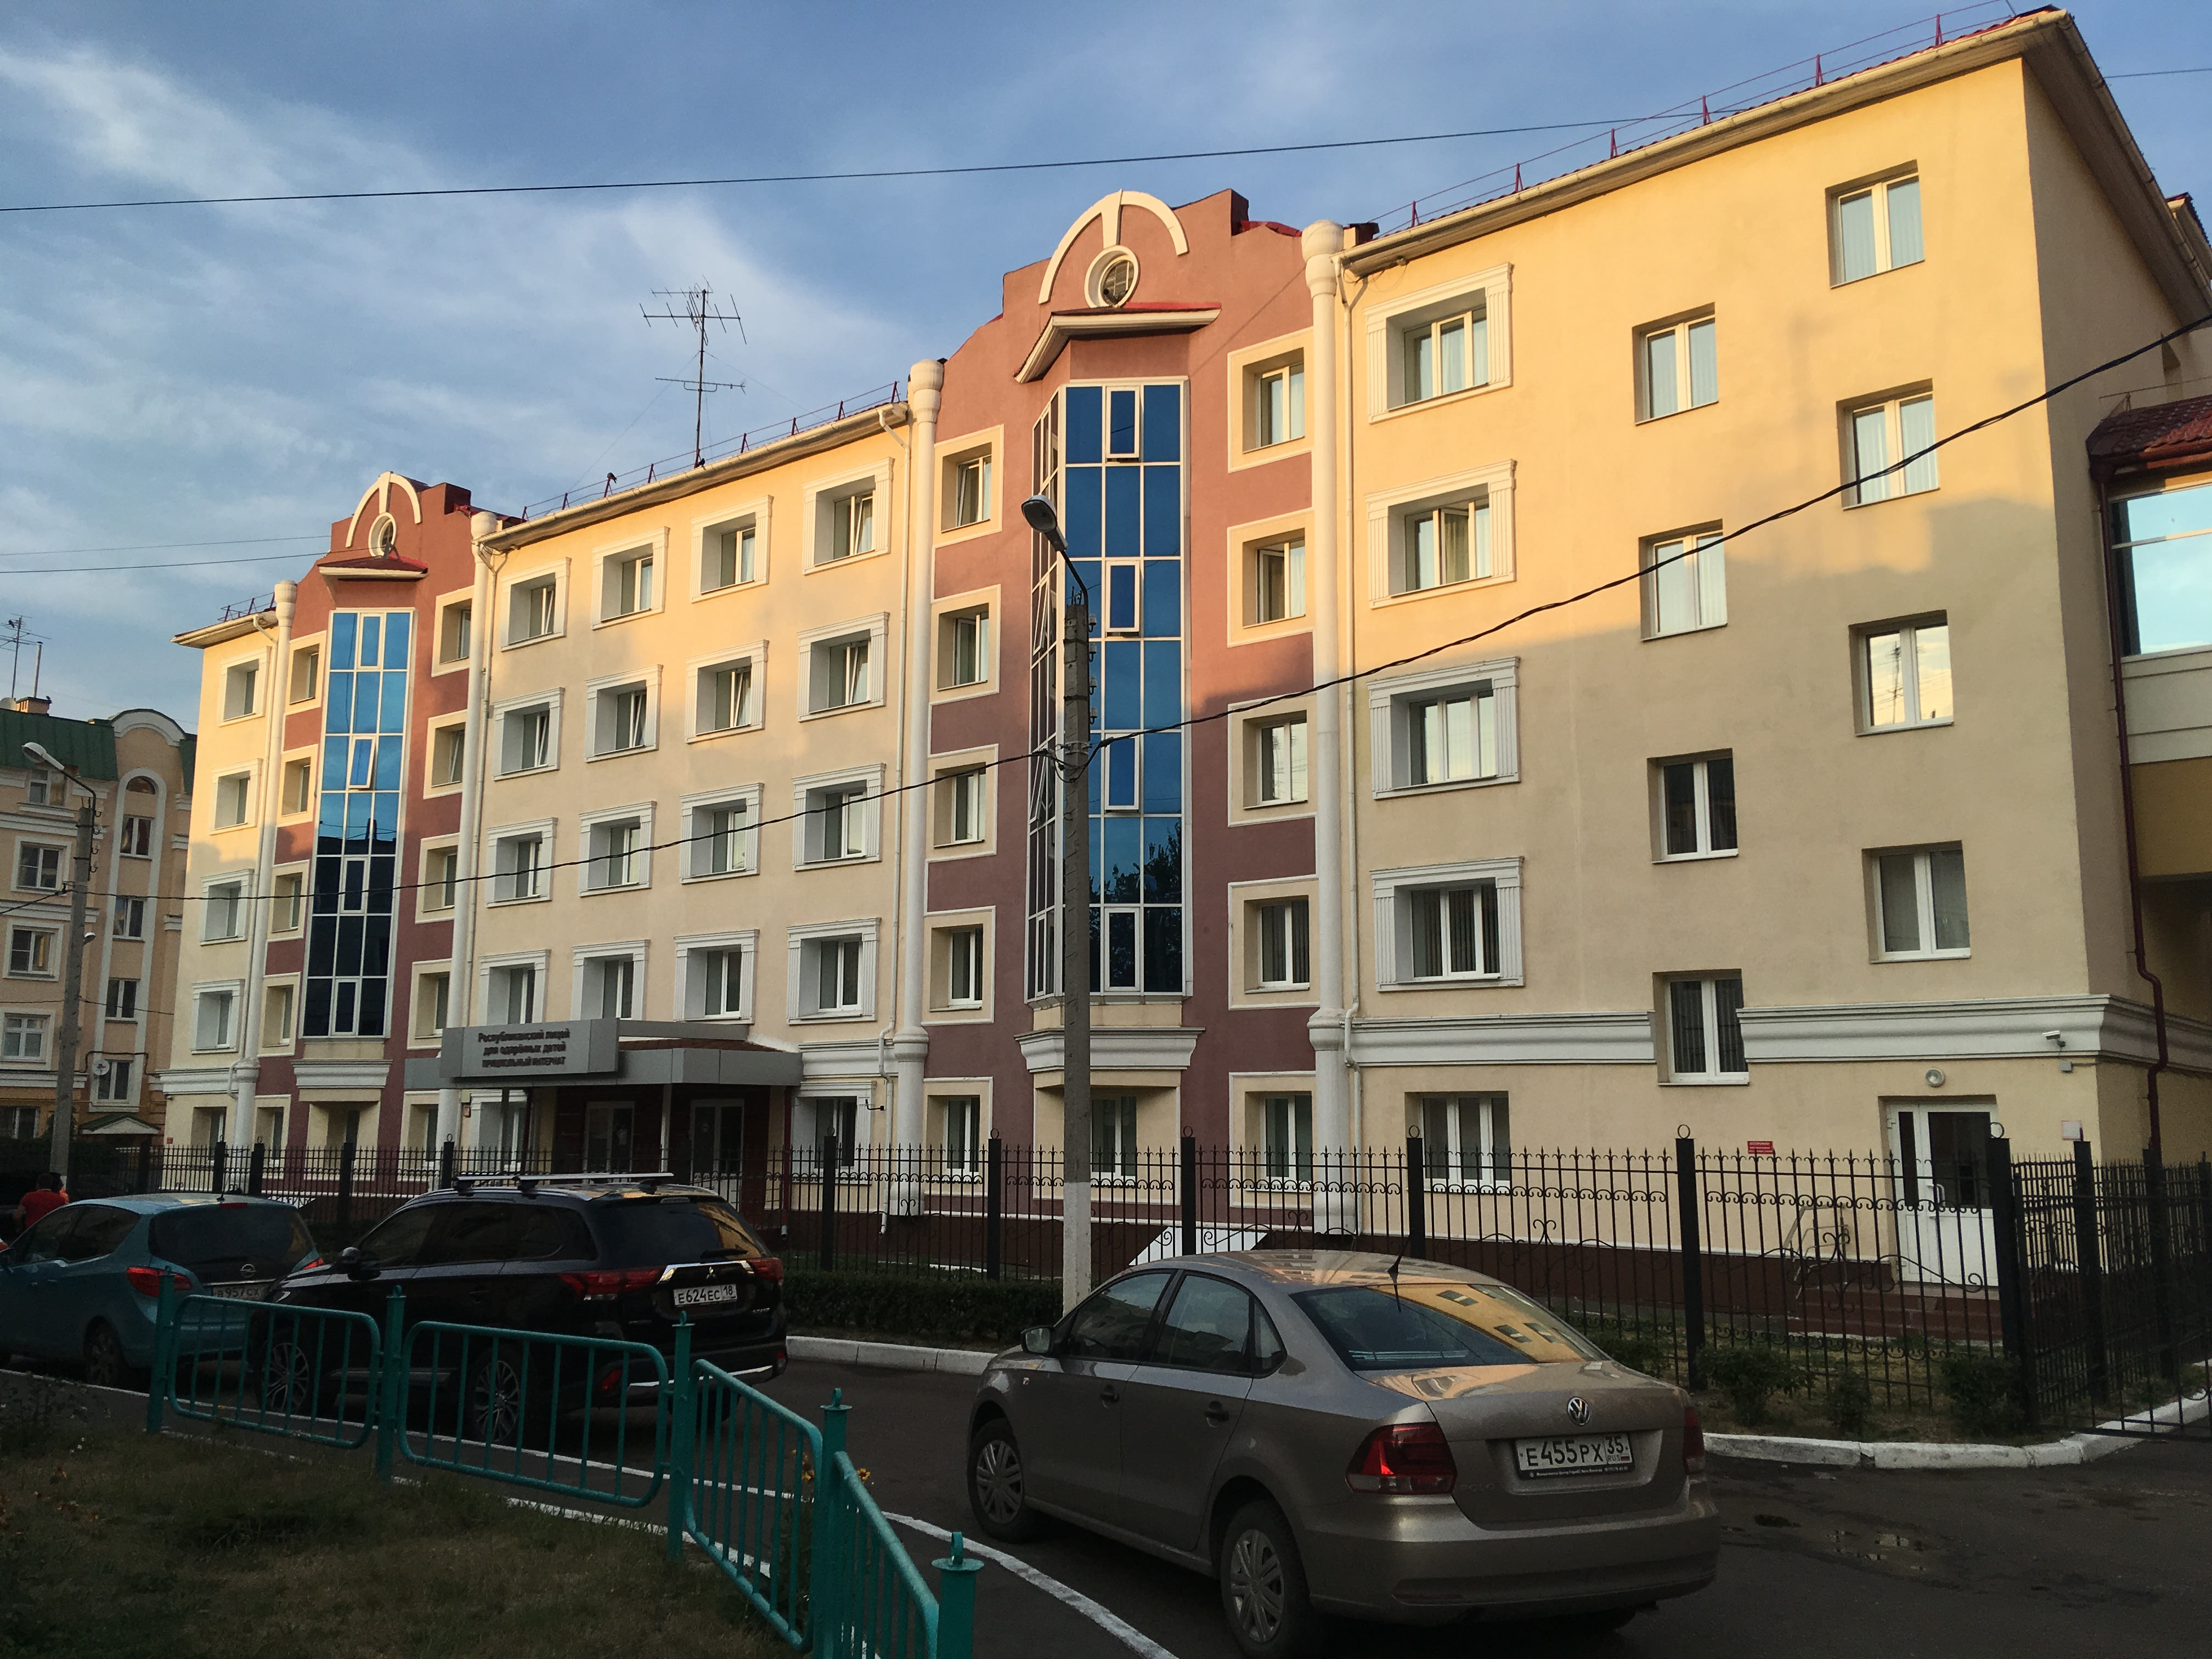
\includegraphics[width=\linewidth]{11}
		\caption{Le dortoir où j'ai vécu pendant 4 ans au lycée de physique et de mathématiques}
		\label{fig:image1}
	\end{minipage}
	\hfill
	\begin{minipage}{0.3\textwidth}
		\centering
		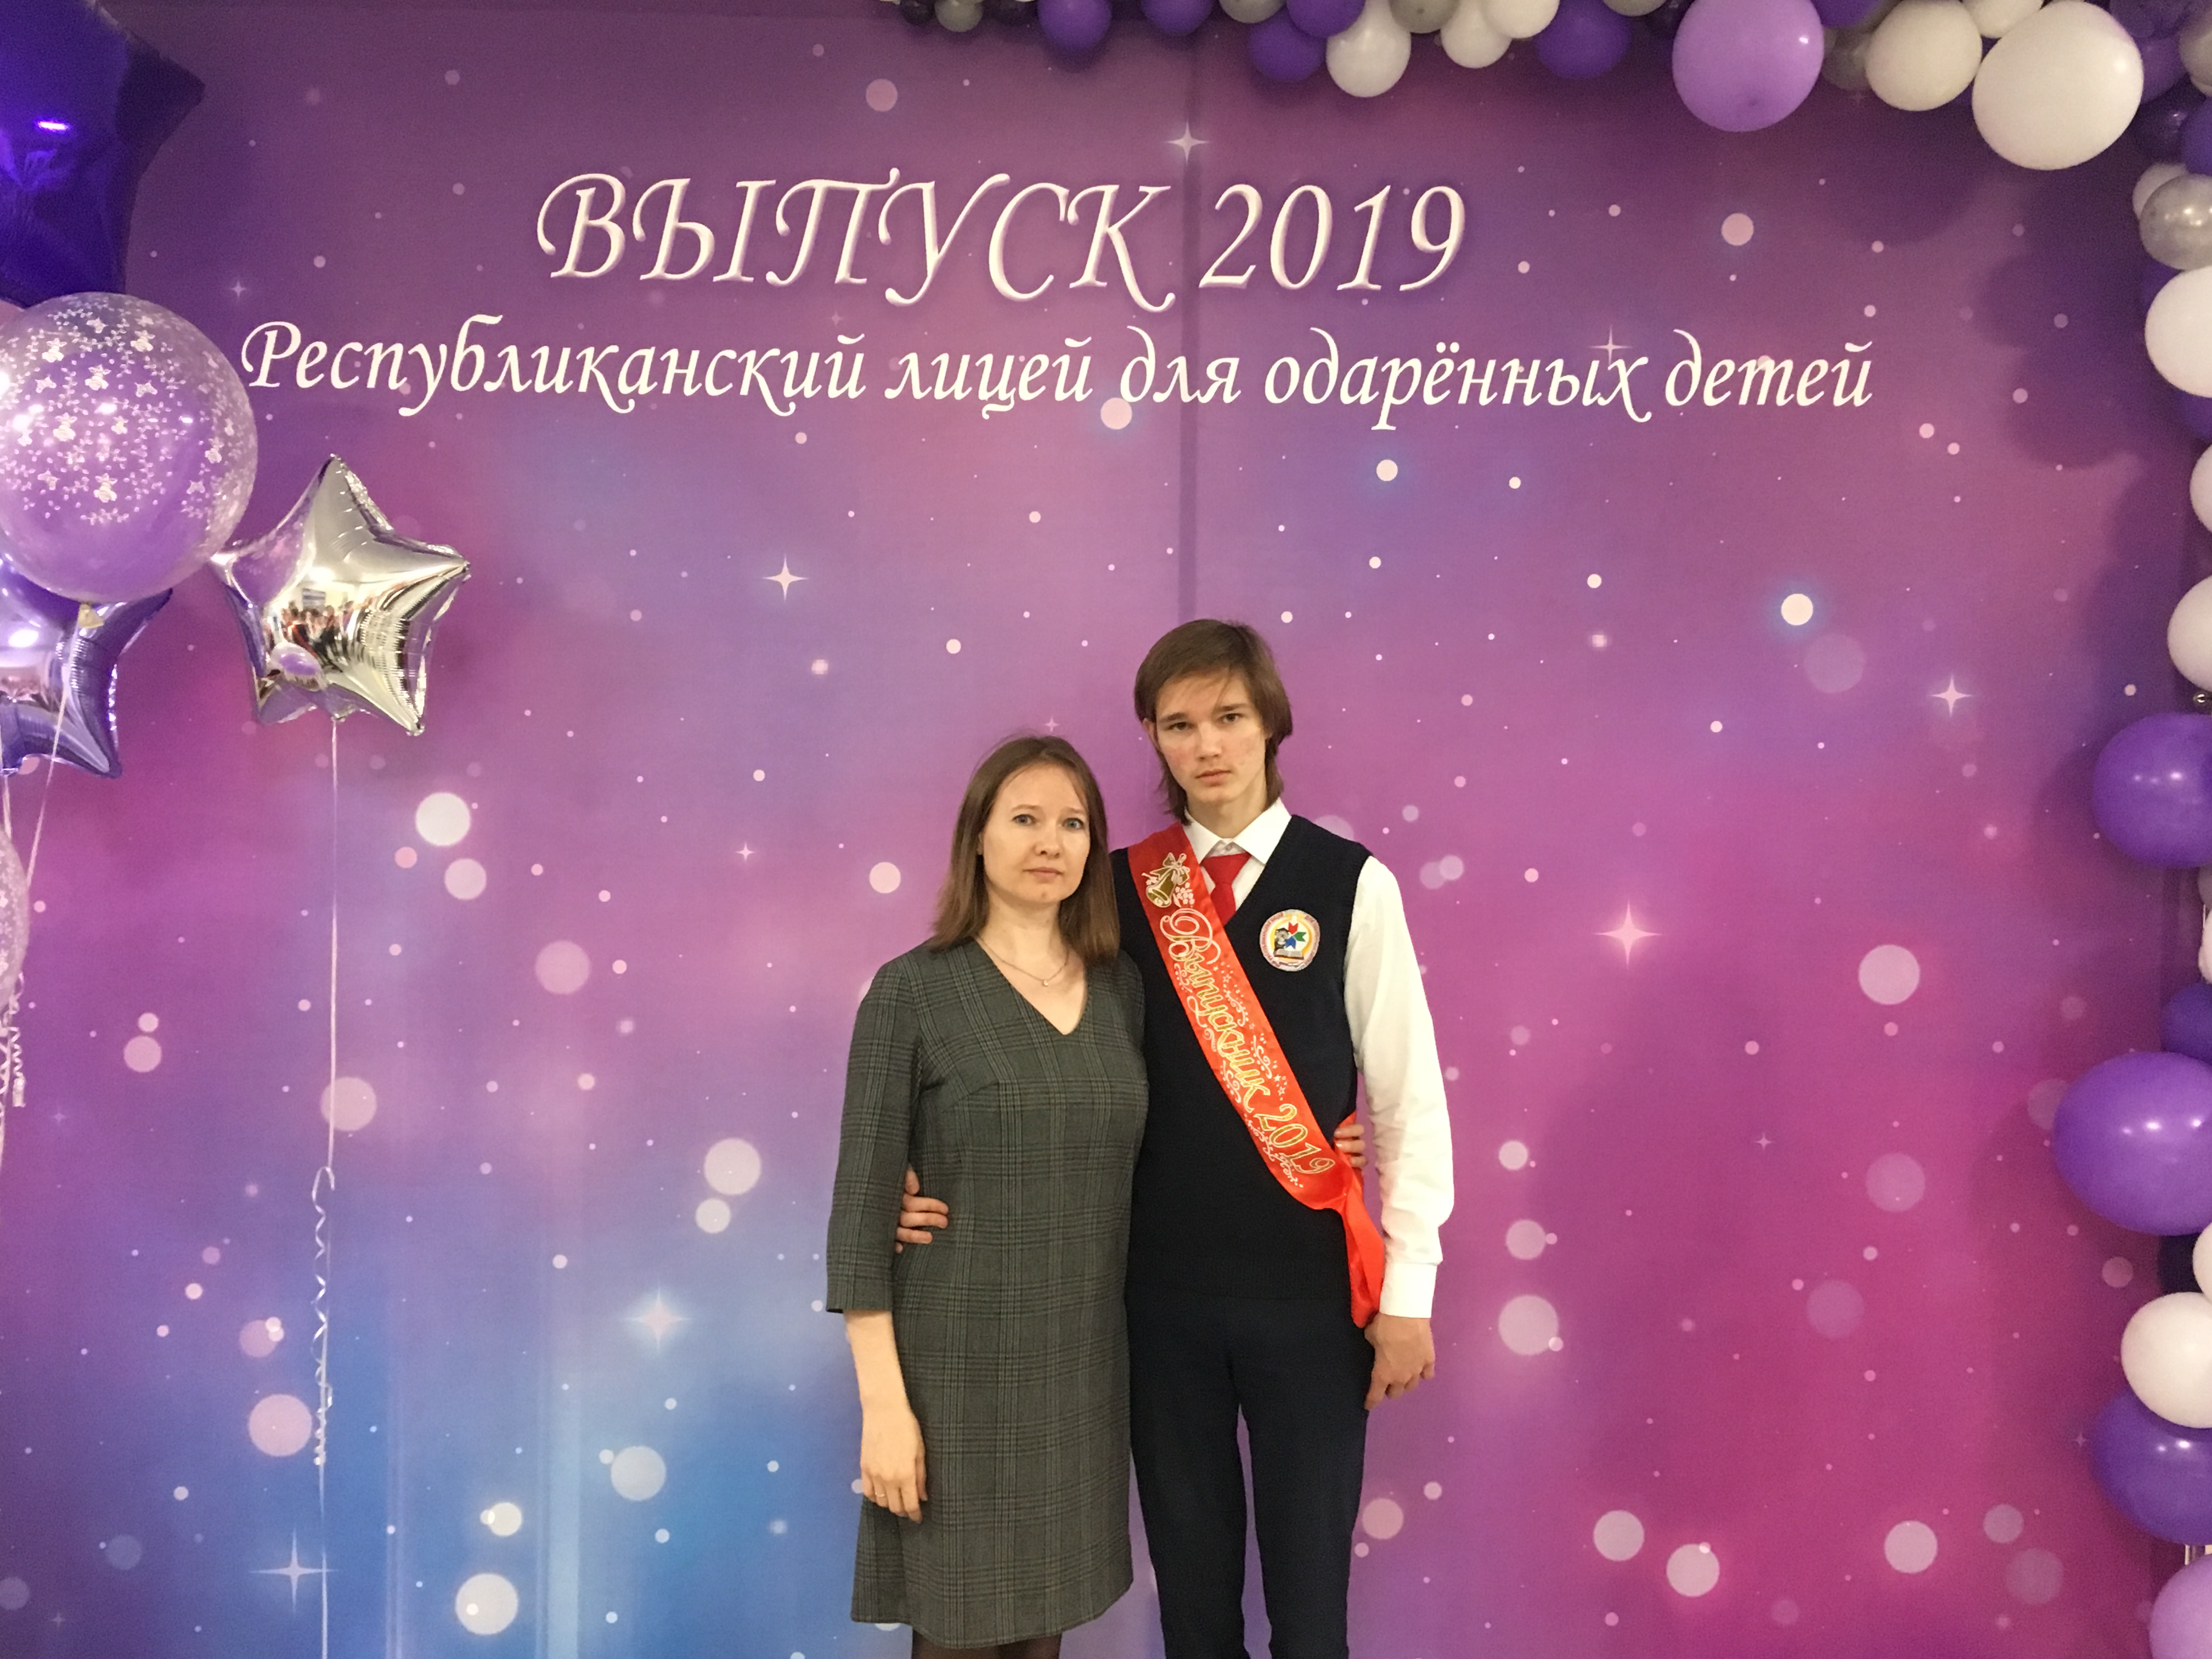
\includegraphics[width=\linewidth]{12}
		\caption{Moi et ma mère à la cérémonie de remise des diplômes du baccalauréat}
		\label{fig:image2}
	\end{minipage}
	\hfill
	\begin{minipage}{0.3\textwidth}
		\centering
		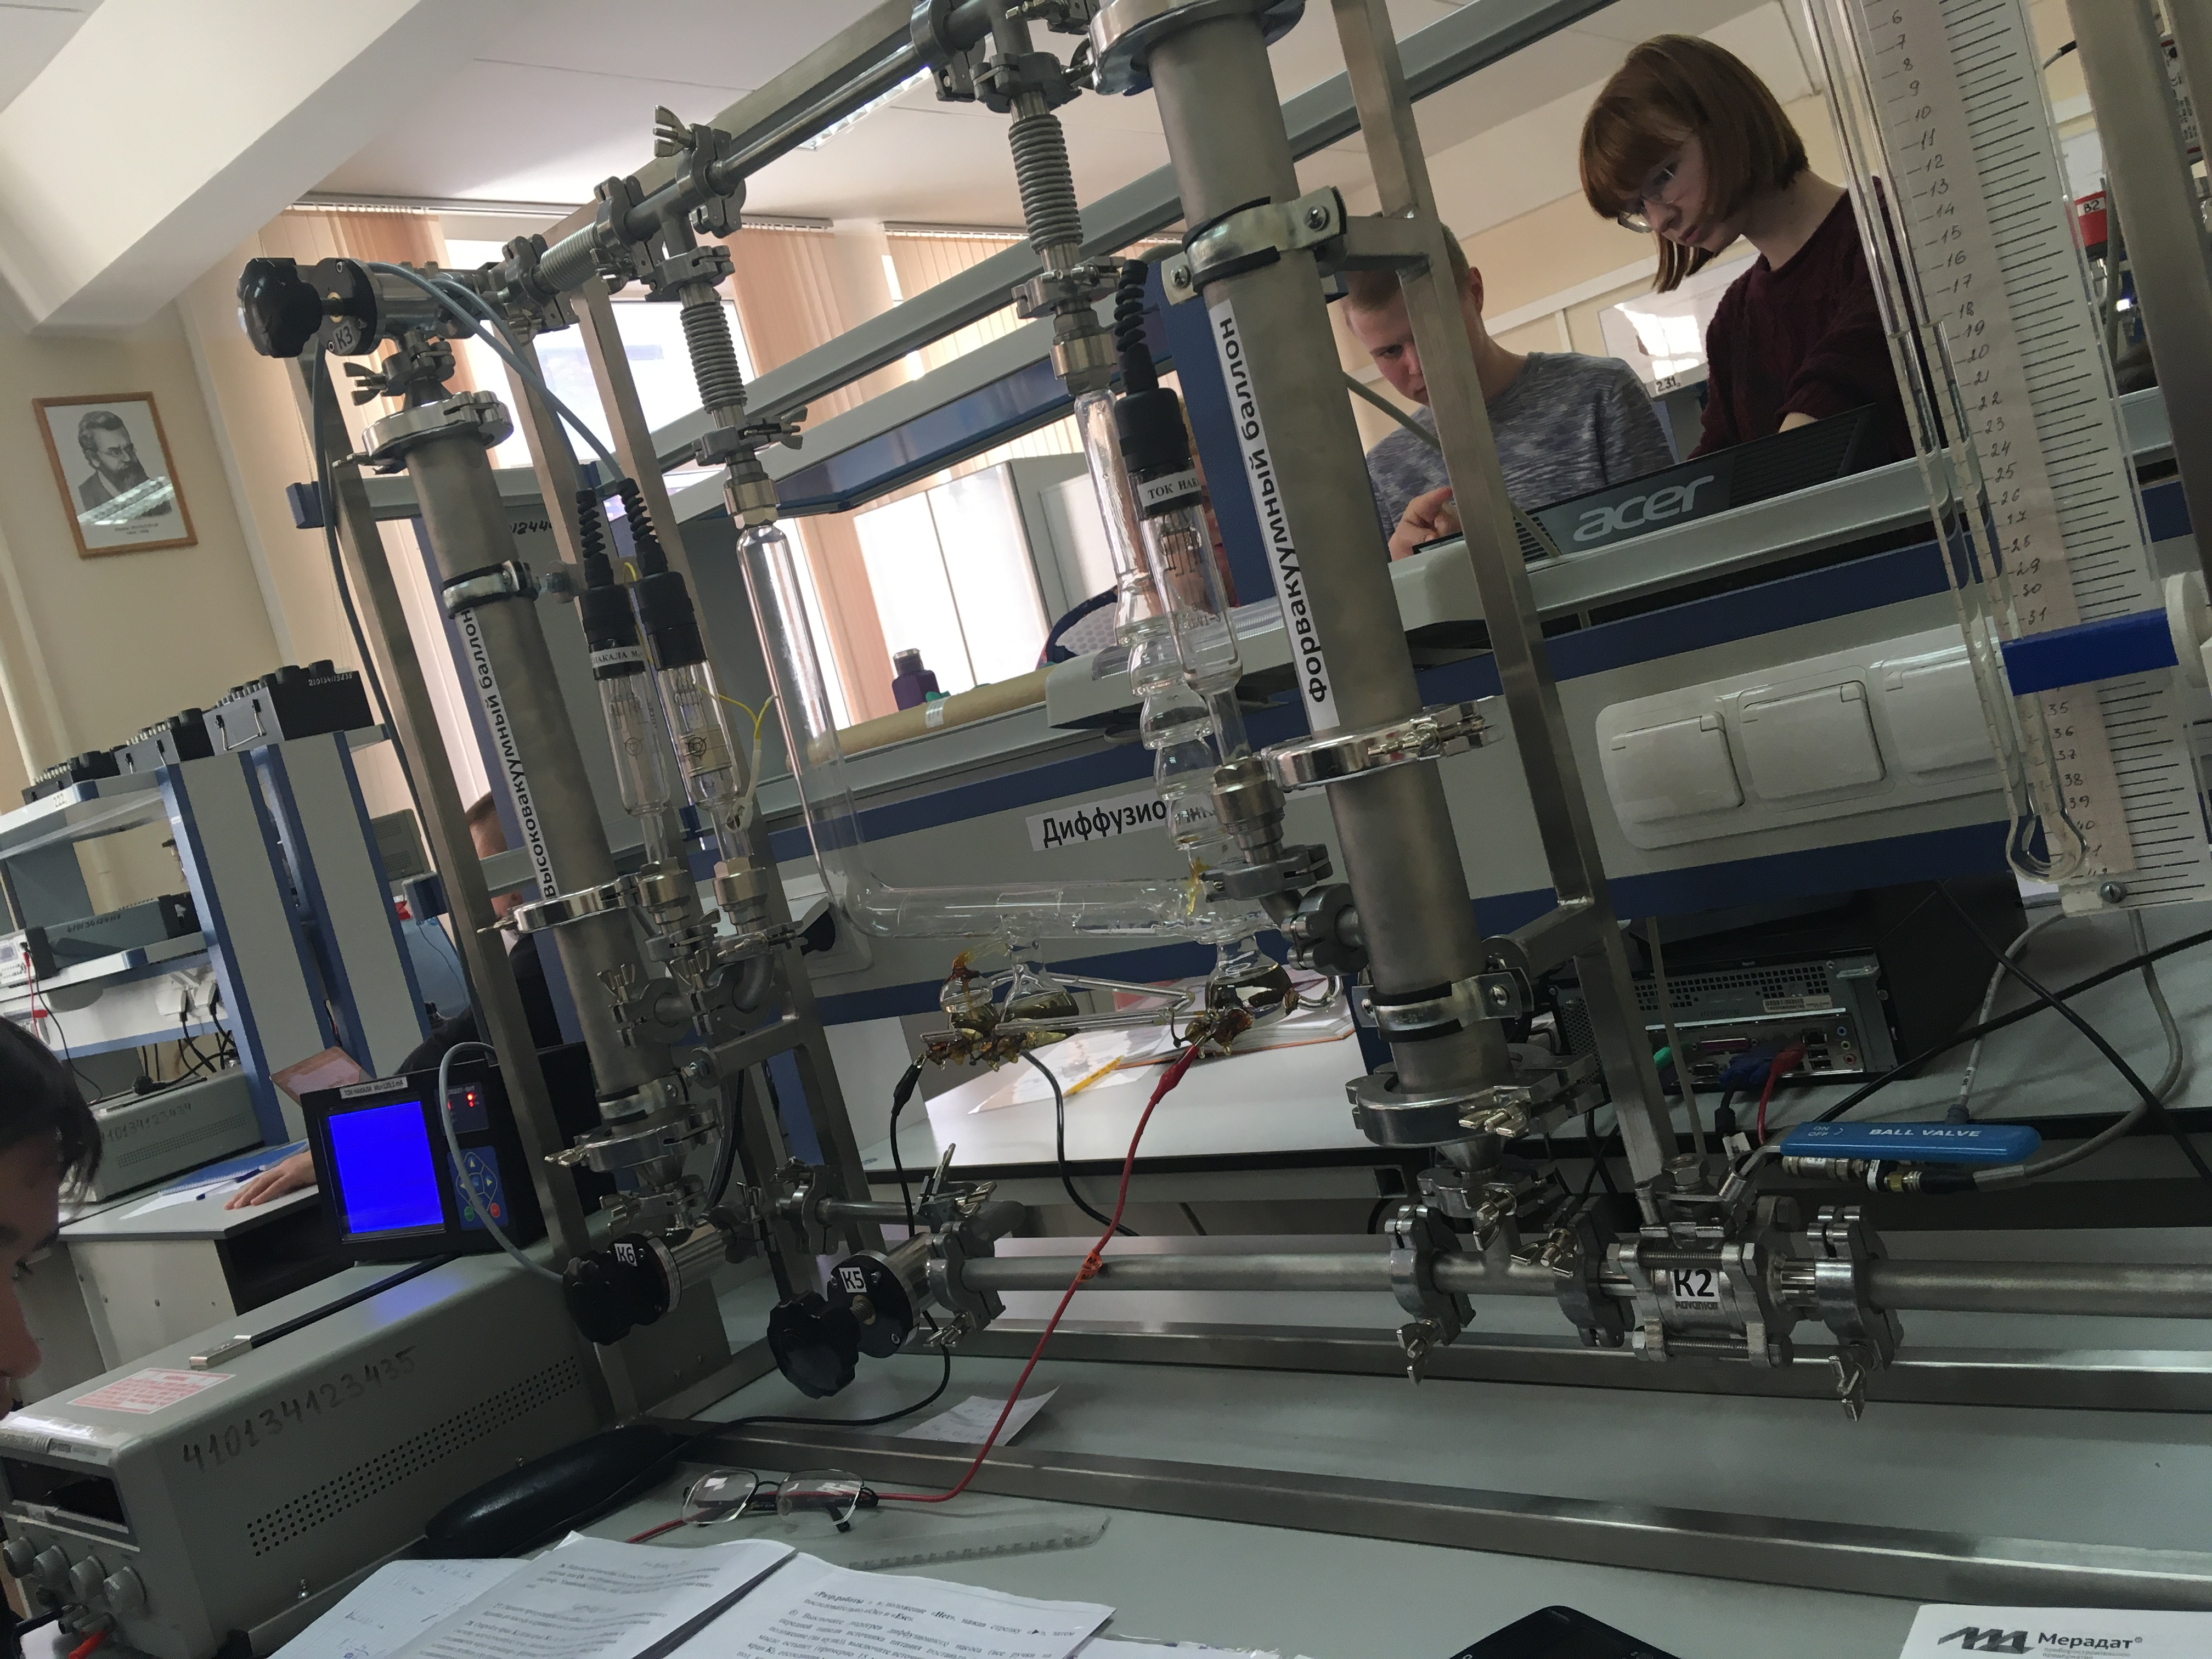
\includegraphics[width=\linewidth]{13}
		\caption{Installation sur laquelle j'ai travaillé pour déterminer le coefficient de diffusion des huiles}
		\label{fig:image3}
	\end{minipage}
	\label{fig:myfigure}
\end{figure}

\section{Expérience française}

Lorsque je suis arrivée en France, j'ai effectué un stage dans le sud de la France afin d'étudier le français de manière intensive et de m'immerger dans la culture et la formation préparatoire, de m'immerger dans l'environnement de l'École Polytechnique et dans ma culture scientifique en français et d'améliorer mon français afin de passer l'examen. C'était l'une des expériences les plus importantes, les plus intéressantes et les plus intenses de ma vie, au cours de laquelle j'ai beaucoup appris et je suis peut-être devenue une personne différente. Je détaille ci-dessous chaque activité, mes progrès et mes observations.

\subsection{Description du parcours effectué (principales activités) depuis mon arrivée en France. Qu’est-ce que j'ai fait et qu’en ai-je pensé?}

Avant mon arrivée en France, j'ai commencé à apprendre le français et à m'habituer à écrire en alphabet latin. J'ai lu un livre assez âgé avec des dialogues en français, ce qui m'a aidé à comprendre la France et la langue française, et qui m'a peut-être encore plus aidé pendant mon stage. Mais je n'ai pas du tout pratiqué la compréhension orale. À mon avis, apprendre le français consiste à apprendre deux langues différentes, le français oral et le français écrit, en raison du système syllabique de la langue, qui n'est pas évident pour les russophones. Le premier mois, malgré mon potentiel en grammaire et en vocabulaire, j'ai eu du mal à comprendre le français à l'oreille.

\subsection{Stage à Villeneuve sur Lot}


J'ai passé 4 mois en stage à Villeneuve, travaillant mon français tous les jours. L'idée de ce stage était que l'étudiant soit immergé dans la culture et la langue grâce à la famille dans laquelle il vit, en plus des cours de français spéciaux combinés à différentes activités. 

Je voudrais dire que pour moi, le stage s'est très bien passé, car j'ai appris un nouveau pays exceptionnel et j'ai validé mon niveau B2, ce qui m'a permis d'acquérir les bases d'un apprentissage autonome de la langue. 


\subsubsection{Famille Morival}

Pendant ces quatre mois, j'ai vécu dans ma famille d'accueil avec Patrick, le grand-père français, et André, un autre étudiant, mon collègue brésilien. Je me souviendrai de cette période comme l'une des plus agréables de ma vie. Et pour cela, je suis très reconnaissant à Patrick. Patrick nous a fait nous sentir comme chez nous en nous accueillant chaleureusement. Il a créé une atmosphère très conviviale pour nous en nous racontant de nombreuses histoires sur sa vie, en partageant sa vie et en faisant de petites visites dans la ville et dans le sud de la France. Patrick nous a traités comme ses petits-enfants qui avaient oublié le français et j'étais même embarrassée qu'il soit si gentil. La dernière fois que j'ai ressenti le même niveau de confort, c'était lorsque ma grand-mère s'occupait de moi, ce qui remonte à loin puisque je vis seule depuis l'âge de 15 ans. 
Ce n'est pas seulement Patrick qui a été si gentil avec nous, mais aussi tous ses amis et connaissances. Lors des apéritifs, des dîners ou des fêtes que nous organisions avec les amis de Patrick, nous faisions toujours partie intégrante de l'événement. On nous parlait, on riait, on plaisantait, on nous nourrissait et on se rappelait de nous. 
Grâce à Patrick, je connais maintenant les traditions de la cuisine française, les différences entre les cuisines des différentes régions de France, les traditions des fêtes, l'organisation politique de la France.\\
En conclusion, Patrick a fait beaucoup pour moi en tant que personne, en changeant ma perception de la gentillesse des autres, pour mes progrès en français, parce qu'il était toujours prêt à parler de n'importe quel sujet et pour ma compréhension de la France. 

\subsubsection{Enseignement à l'IFLS.}

Je voudrais maintenant aborder plus en détail le style d'enseignement de l'IFLS. J'ai étudié l'anglais pendant environ 6 ans et en comparant mon expérience d'apprentissage de l'anglais et du français, je peux dire que toutes les conditions nécessaires, telles qu'un retour d'information rapide et un intérêt extérieur pour les sujets traités en français, ont été réunies pour permettre de grands progrès. Nos groupes étaient encadrés par trois professeurs, Lucy, Sophie et Marion, ainsi que par la directrice de l'école, qui donnait des conférences thématiques sur la France. Chaque professeur était responsable d'un des groupes répartis par niveau de langue. J'étais dans le groupe du milieu, parce qu'apparemment je parlais un peu, mais à la fin du stage, à mon avis, la différence entre nos groupes avait presque disparu, grâce au charisme et à l'approche unique de chacune des professeures. Chacune d'entre elles a choisi des supports d'écoute, de lecture, d'expression orale de manière indépendante, et tous ont été mémorables, raison pour laquelle je garde toutes les feuilles de nos cours dans un ordre trié, de sorte que peut-être un jour je reviendrai et relirai nos textes de littérature de fiction. Marion a toujours choisi d'excellents ouvrages qui m'ont poussé à apprendre le français d'une bonne manière, car je me sentais faible, incapable de comprendre un excellent texte. Lucy choisissait des articles de faits divers intéressants, des nouvelles et des oraux très captivants. Sophie, qui était responsable de notre groupe, a excellé dans tous les domaines, y compris en grammaire. Je me souviendrai probablement toute ma vie de la merveilleuse compréhension orale de madeleine de Proust par Sophie, que nous avons faite par la suite. Le fait que Sophie se préoccupe de notre niveau de langue, qu'elle nous donne des informations précieuses et qu'elle nous prépare très bien aux leçons était très motivant. J'aimerais souligner qu'en plus de parler à Patrick, Sophie m'a fait énormément progresser avec les expressions écrites, car les sujets étaient très importants et je voulais écrire des centaines de mots dessus. Elle m'a également donné un sentiment d'individualité dans le feedback, en soulignant chaque erreur et en décrivant les progrès et les points à surveiller.

À la fin de mes études avec les professeurs de l'IFLS, je peux dire que j'ai fait de grands progrès en français grâce à l'environnement unique et au système d'enseignement unique, car lorsque je suis arrivé en France, je savais à peine parler français. Après lui, je peux dire avec confiance que j'ai atteint un niveau qui me permet de progresser seul avec les bases données à l'IFLS. 

\subsubsection{Club Alpin}

Pendant notre temps libre, une fois par semaine, nous devions nous rendre dans un club pour progresser en français de plus en plus. On nous a donné une liste d'organisations complètement différentes, du club d'échecs au musée de Villeneuve. À ce moment-là, je voulais trouver un nouveau loisir, comme l'escalade, et j'ai donc fréquenté une section particulière que j'ai trouvée par moi-même : le club alpin français d'alpinisme du Lot et Garonne. Il constitue un réseau de clubs d'escalade dans toute la France et j'ai eu la chance de le trouver dans une si petite ville. Le club était un grand bâtiment historique équipé d'une immense salle avec des murs d'escalade et tout l'équipement nécessaire. Chaque soir ouvrable, la salle était presque toujours remplie des mêmes personnes, les membres du club qui créaient une atmosphère sportive chaleureuse. En participant à ce club, il semble que j'ai dépassé mon niveau de confort, car il m'était très difficile de comprendre le français dans des situations stressantes en altitude, dans lesquelles je ne savais pas quoi dire, même en russe, parce que je n'avais jamais fait d'escalade. Mais en fin de compte, j'ai été très heureuse de mon choix, car les membres du club étaient des interlocuteurs très intéressants, des grimpeurs amateurs et des professionnels passionnés.


%	
\subsection{Formation préparatoire}

Après avoir terminé mon stage dans le sud de la France, je suis retourné à l'École Polytechnique pour la formation préparatoire. Son objectif était de me familiariser avec le système d'enseignement technique en France, de m'habituer à penser scientifiquement en français et de préparer assidûment l'examen du TCF en français. La période de préparation a duré 2 mois sur le campus de l'Ecole polytechnique, on peut ainsi dire que j'ai commencé à étudier avec 2 mois d'avance. 

Pendant ces deux mois, j'ai amélioré mon français de manière très significative en validant mon niveau C1 et en apprenant à expliquer mes connaissances techniques en français.
 
\subsubsection{Les cours scientifiques}

J'ai suivi un cours d'algèbre linéaire, d'analyse mathématique sous différentes formes, de mécanique quantique à partir des concepts de base, qui ont progressé très rapidement au fur et à mesure que nous arrivions au niveau du TC, plus proche des derniers cours. Cela s'est avéré très utile, car je connaissais la majeure partie de la matière, mais je ne savais pas comment exprimer mes connaissances. 

Dans nos cours, nous avons également beaucoup insisté sur les spécificités françaises de la notation et sur la manière de présenter les devoirs. Pour moi qui suis capable de changer très rapidement le fil de mes pensées, c'était quelque chose de nouveau, car j'écris vite et pas vraiment proprement, mais de manière efficace en termes de résolution de problèmes. Je peux dire qu'on m'a même appris de cette manière, lorsque je faisais les Olympiades et les examens du MIPT, à donner la priorité à la solution du problème sous contrainte de temps et à me battre pour mon bon droit si la pensée n'est pas comprise. 

Dans le système français, il faudrait que je me réhabitue à une manière de résoudre plus détendue, plus ordonnée, tout en gardant mon efficacité. 

Je voudrais également souligner l'abondance du matériel et l'originalité de la présentation. Tout d'abord, chaque cours avait son propre manuscrit d'auteur et ses grandes lignes sous la forme de présentations ou d'une sélection unique de tâches pour une meilleure compréhension de la matière. Deuxièmement, après chaque PC, il était toujours possible de revenir aux solutions si je n'étais pas sûr d'avoir compris l'ensemble du sujet. Dans un environnement où je comprenais absolument les formules sur le tableau, mais pas jusqu'au bout de ma pensée, cela s'est avéré très efficace. 

\subsubsection{Les cours du français}

Comme l'un des principaux objectifs était de réussir un examen impliquant la confirmation de mon diplôme, nous avons eu des cours de français très intensifs, présentés dans tous les types d'expressions.

Pour améliorer l'écriture avec le professeur de grammaire Frédéric Valat, j'ai écrit de courts textes en mettant l'accent sur mon point de vue. Par exemple, dans une lettre, je devais évaluer la réforme des écoles canadiennes et donner mon avis. J'aimerais mentionner une lettre créative que nous avons réalisée en groupe avec une petite présentation. De la même manière que Perec, je devais écrire un texte décrivant ce qui se passe à Paris dans n'importe quel endroit bondé, comme il l'a fait lui-même dans un café. 

De plus, par rapport au stage dans le sud, nous avons eu des séances de conversation tout à fait uniques avec un professeur dans un petit groupe où nous avons discuté assez vigoureusement de questions philosophiques sur l'art et amélioré notre prononciation. 

En combinant l'abondance culturelle de Paris avec l'apprentissage de la langue, nous avons réussi à faire 3 visites culturelles au musée d'art et une promenade guidée dans les sites historiques du Quartier Latin, où nous avons également dû préparer de petites présentations sur les sites historiques pour tout le groupe. Malheureusement, nous n'avons pas pu faire deux autres visites dans le cadre des grèves qui se déroulaient à Paris à ce moment-là. 

L'un des éléments qui a le plus contribué à améliorer mon niveau de français a été le cours intensif de préparation au TCF avec Margaux Duval, au cours duquel j'ai noté, à chaque session, une centaine de phrases de niveau avancé. Au cours des premières semaines, elle a calibré nos cours non pas en fonction de notre niveau actuel, mais en fonction d'un niveau à atteindre, de sorte qu'à chaque session, je me sentais hors de ma zone de confort. Cela m'a motivé à y retourner chaque fois pour en apprendre toujours plus. Je crois qu'en faisant attention à ces petites choses, j'ai progressé assez rapidement à moyen terme. 

\subsection{Quels difficultés ai-je rencontré? Quels sont mes réussites et échecs?}

En comparant mes attentes et la réalité, je peux dire que mon intégration a été très réussie. Je n'ai pas eu de problèmes d'intégration, ni de problèmes de non-acceptation dans une nouvelle société. On a toujours été disposé à me parler, voire même à me contacter, même si j'avais l'impression que c'était à moi de prendre l'initiative. Bien sûr, à de nombreuses occasions, j'ai pris l'initiative de prouver que j'étais capable de maintenir un dialogue et d'exprimer mes pensées, mais lorsque c'était clair de visu, je n'ai pratiquement pas eu de problèmes de non-acceptation.  

Je peux dire qu'au début, lorsque j'avais des problèmes de compréhension orale ou de choix de mots, je sentais moi-même que je ne pouvais pas être acceptée dans la nouvelle société. Une nouvelle société ne peut pas m'accepter si je n'en fais pas partie à part entière. Comprenant cela, j'ai toujours essayé de réduire la distance autant que possible par des compétences linguistiques, et simplement par des points communs. 

J'ai donc travaillé mon vocabulaire et ma connaissance de la France, par exemple l'histoire et la cuisine. Je voudrais également mentionner l'accent et la prononciation. Un accent est un trait unique, un peu comme un compliment à l'égard d'une personne, c'est un attribut de sa culture. Il n'est peut-être pas nécessaire de se débarrasser d'un accent si vous n'utilisez la langue qu'à des fins professionnelles. Cependant, à mon avis, pour s'intégrer, il faut adopter la prononciation naturelle de la langue. Cependant, à mon avis, pour s'intégrer, il faut adopter la prononciation naturelle dans la langue. De plus, le niveau de la langue semble plus élevé si l'on parle de manière claire et structurée, même avec des erreurs. 

Pour conclure, il est évident que je ne comprends pas le contexte de ce que les Français ont vécu, ce qui rend parfois l'intégration difficile. Par exemple, les événements qui ont eu lieu en France, dont je ne suis pas au courant, ou simplement l'argot. Mais en même temps, je comprends que dans une large mesure, seul mon travail sur moi-même et mon séjour en France peuvent au moins partiellement aplanir cet angle. 


\subsection{Soft skills}
%	
\subsubsection{Mes réflexions sur les compétences de convaincre}

Lors de chaque représentation, je réfléchis constamment à ma capacité de convaincre. Et je pense que j'ai mon propre style de persuasion. Lorsque je suis sur scène, même devant un petit public, je me sens mal à l'aise dans mes mouvements, je peux agiter mon bras de manière assez maladroite et brusque, ce qui ajoute à l'effet de surprise et détourne l'attention de l'histoire plutôt que de persuader. Mais j'essaie de mettre l'accent sur ce que je dis. J'essaie de bien comprendre l'histoire que je vais raconter si je ne la connais pas assez pour la connaître par cœur. C'est-à-dire que je deviens un peu un expert local. Je trouve que la confiance en ce que je dis et un avis critique d'expert impressionnent à l'intérieur de tout auditeur attentif. J'essaie également, au tout début, de choisir un public pour lequel je parle, afin d'être sûr que mes auditeurs m'écouteront, qu'ils seront intéressés. 
\subsubsection{Évolution de mes points forts et points faibles depuis mon arrivée en France}

Depuis mon arrivée en France, je pense que je suis devenu plus ouvert aux gens. Dans une société assez ouverte, la compréhension et l'ouverture d'esprit qui m'entourent m'ont également transmis ces qualités. Je ne veux pas dire que je n'avais pas ces qualités, peut-être que leur niveau n'a même pas changé, mais j'ai certainement appris à les partager. Autant que possible, j'essaie de participer à toutes les activités de groupe, en particulier celles qui dépassent mon seul intérêt, afin d'établir des liens plus étroits avec les gens. J'ai participé à notre théâtre international d'étudiants à Villeneuve, j'ai donné un petit concert de guitare acoustique et j'ai constamment essayé de m'immerger dans un environnement qui ne m'était pas familier, du mieux que je pouvais. Le besoin de m'intégrer semble m'avoir influencé dans ce sens également. Avant même mon arrivée, j'étais conscient que je ne pouvais pas rester fermé et ne communiquer qu'avec un petit cercle de personnes, sinon je n'aurais pas pu apprendre la langue. 





	\section{Projets pour l'avenir}
	\subsection{Quelles sont les options scientifiques à l’X pour la suite de mes projets?}
	Je pense que je m'intéresserai de plus en plus à l'informatique et à l'apprentissage profond, car j'ai déjà fait un choix approximatif du domaine que je veux poursuivre. C'est plus facile pour moi, car je sauterai sur toutes les occasions de réaliser un projet informatique et je prendrai mes initiatives et mes idées de projets, parce que je les ai déjà. Par exemple, tester et développer de nouvelles architectures pour toutes sortes de traitements de données, y compris des images ou des enregistrements audio. 
	
	Il faut aussi être conscient de sa culture et que les idées peuvent venir d'ailleurs que de son cœur de métier. Par exemple, pour comprendre les fonctions eurétiques des activations dans les réseaux neuronaux, il faut comprendre le fonctionnement d'un neurone dans un corps vivant, c'est-à-dire le fonctionnement d'une cellule. A cet égard, l'idée d'une formation interdisciplinaire de l'École Polytechnique avec la possibilité d'un aprofondissement en 3ème année me convient parfaitement. 
	\subsection{Le choix de binet}
	Je n'ai pas encore choisi mon binet, mais j'aimerais vraiment choisir un binet en fonction de mes hobbies. Comme j'aime beaucoup la nature et la randonnée, je voudrais rejoindre un binet de montagne, parce qu'il y a surtout des gens qui ne font pas seulement de l'alpinisme ou du ski, mais qui aiment aussi la randonnée. J'aime aussi jouer de la guitare acoustique et de la guitare électrique, c'est pourquoi j'aimerais rejoindre un binet de musique rock. Je suis sûr qu'à en juger par le nombre de binets, il y en a d'autres que je ne connais pas encore, mais que j'aimerais rejoindre. 
	
	\subsection{Vers quelle orientation professionnelle souhaite-je me diriger à court terme et éventuellement à plus long terme?}
	
	À court terme, j'aimerais me concentrer autant que possible sur la connaissance de la pratique de la programmation, c'est-à-dire sur les algorithmes, la théorie et les projets, car les dix prochaines années sont les plus propices aux activités cognitives. Après avoir acquis suffisamment d'expérience dans les projets, j'aimerais gérer moi-même des projets, dans lesquels je pourrais théoriquement m'occuper de tous les détails dans un délai raisonnable. Cela me semble être une étape assez logique, car après chaque projet, on trouve des idées personnelles que l'on aimerait mettre en œuvre. 
%	

	
	\section{Conclusion}

Dans ce rapport, j'ai décrit mon parcours et mon niveau de préparation, le déroulement de mes études à l'École Polytechnique avant le TC et mes projets pour l'avenir. J'ai essayé de couvrir autant que possible les différences culturelles, linguistiques et professionnelles que j'ai rencontrées pendant mon séjour en France et la manière dont je les ai plus ou moins bien gérées. C'était l'un des moments les plus inoubliables de ma vie et je suis sûr que ce ne sera pas le premier à l'École Polytechnique.  

En conclusion, je voudrais souligner une fois de plus ma forte motivation à réaliser mes projets et je voudrais remercier l'École Polytechnique, ses professeurs, ses employés, les organisateurs d'événements, l'atelier pour les opportunités qui m'ont été données.  

\begin{figure}[htbp]
	\centering
	\begin{minipage}{0.3\textwidth}
		\centering
		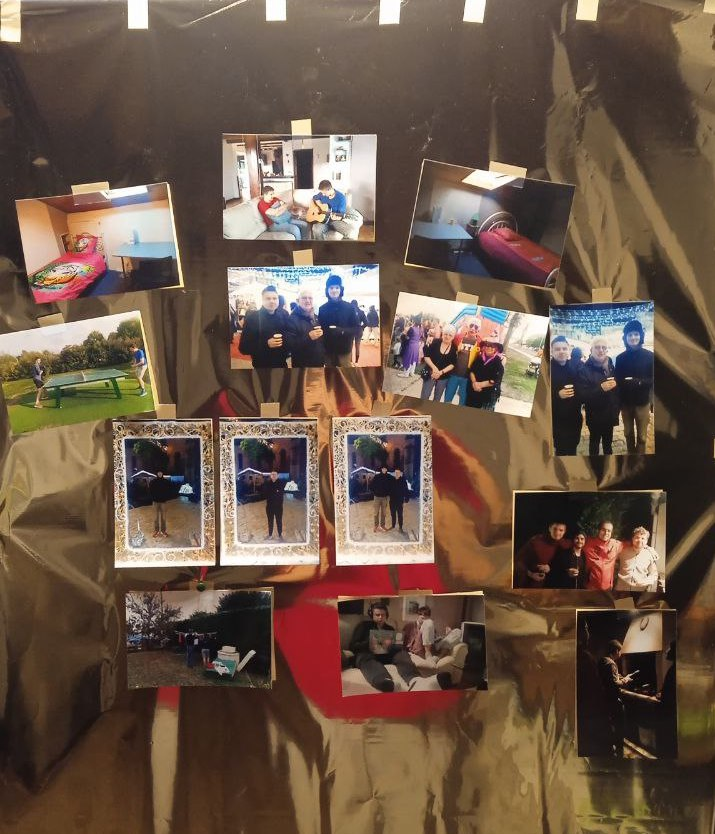
\includegraphics[width=\linewidth]{3}
		\caption{Nos photos que Patrick a accrochées à son mur en souvenir de l'événement.}
		\label{fig:image1}
	\end{minipage}
	\hfill
	\begin{minipage}{0.3\textwidth}
		\centering
		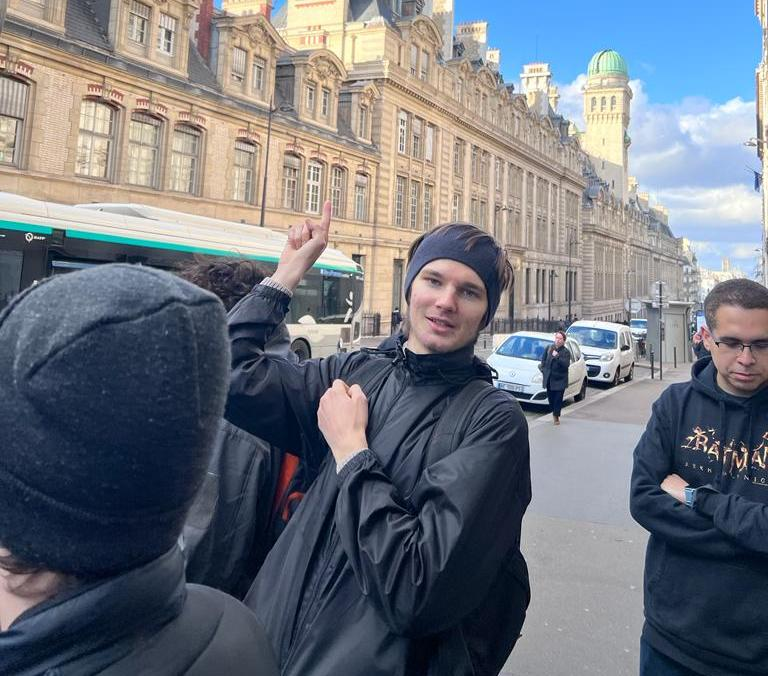
\includegraphics[width=\linewidth]{33}
		\caption{Je montre le mur d'obus lors d'une randonnée dans le Quartier Latin}
		\label{fig:image2}
	\end{minipage}
	\hfill
	\begin{minipage}{0.3\textwidth}
		\centering
		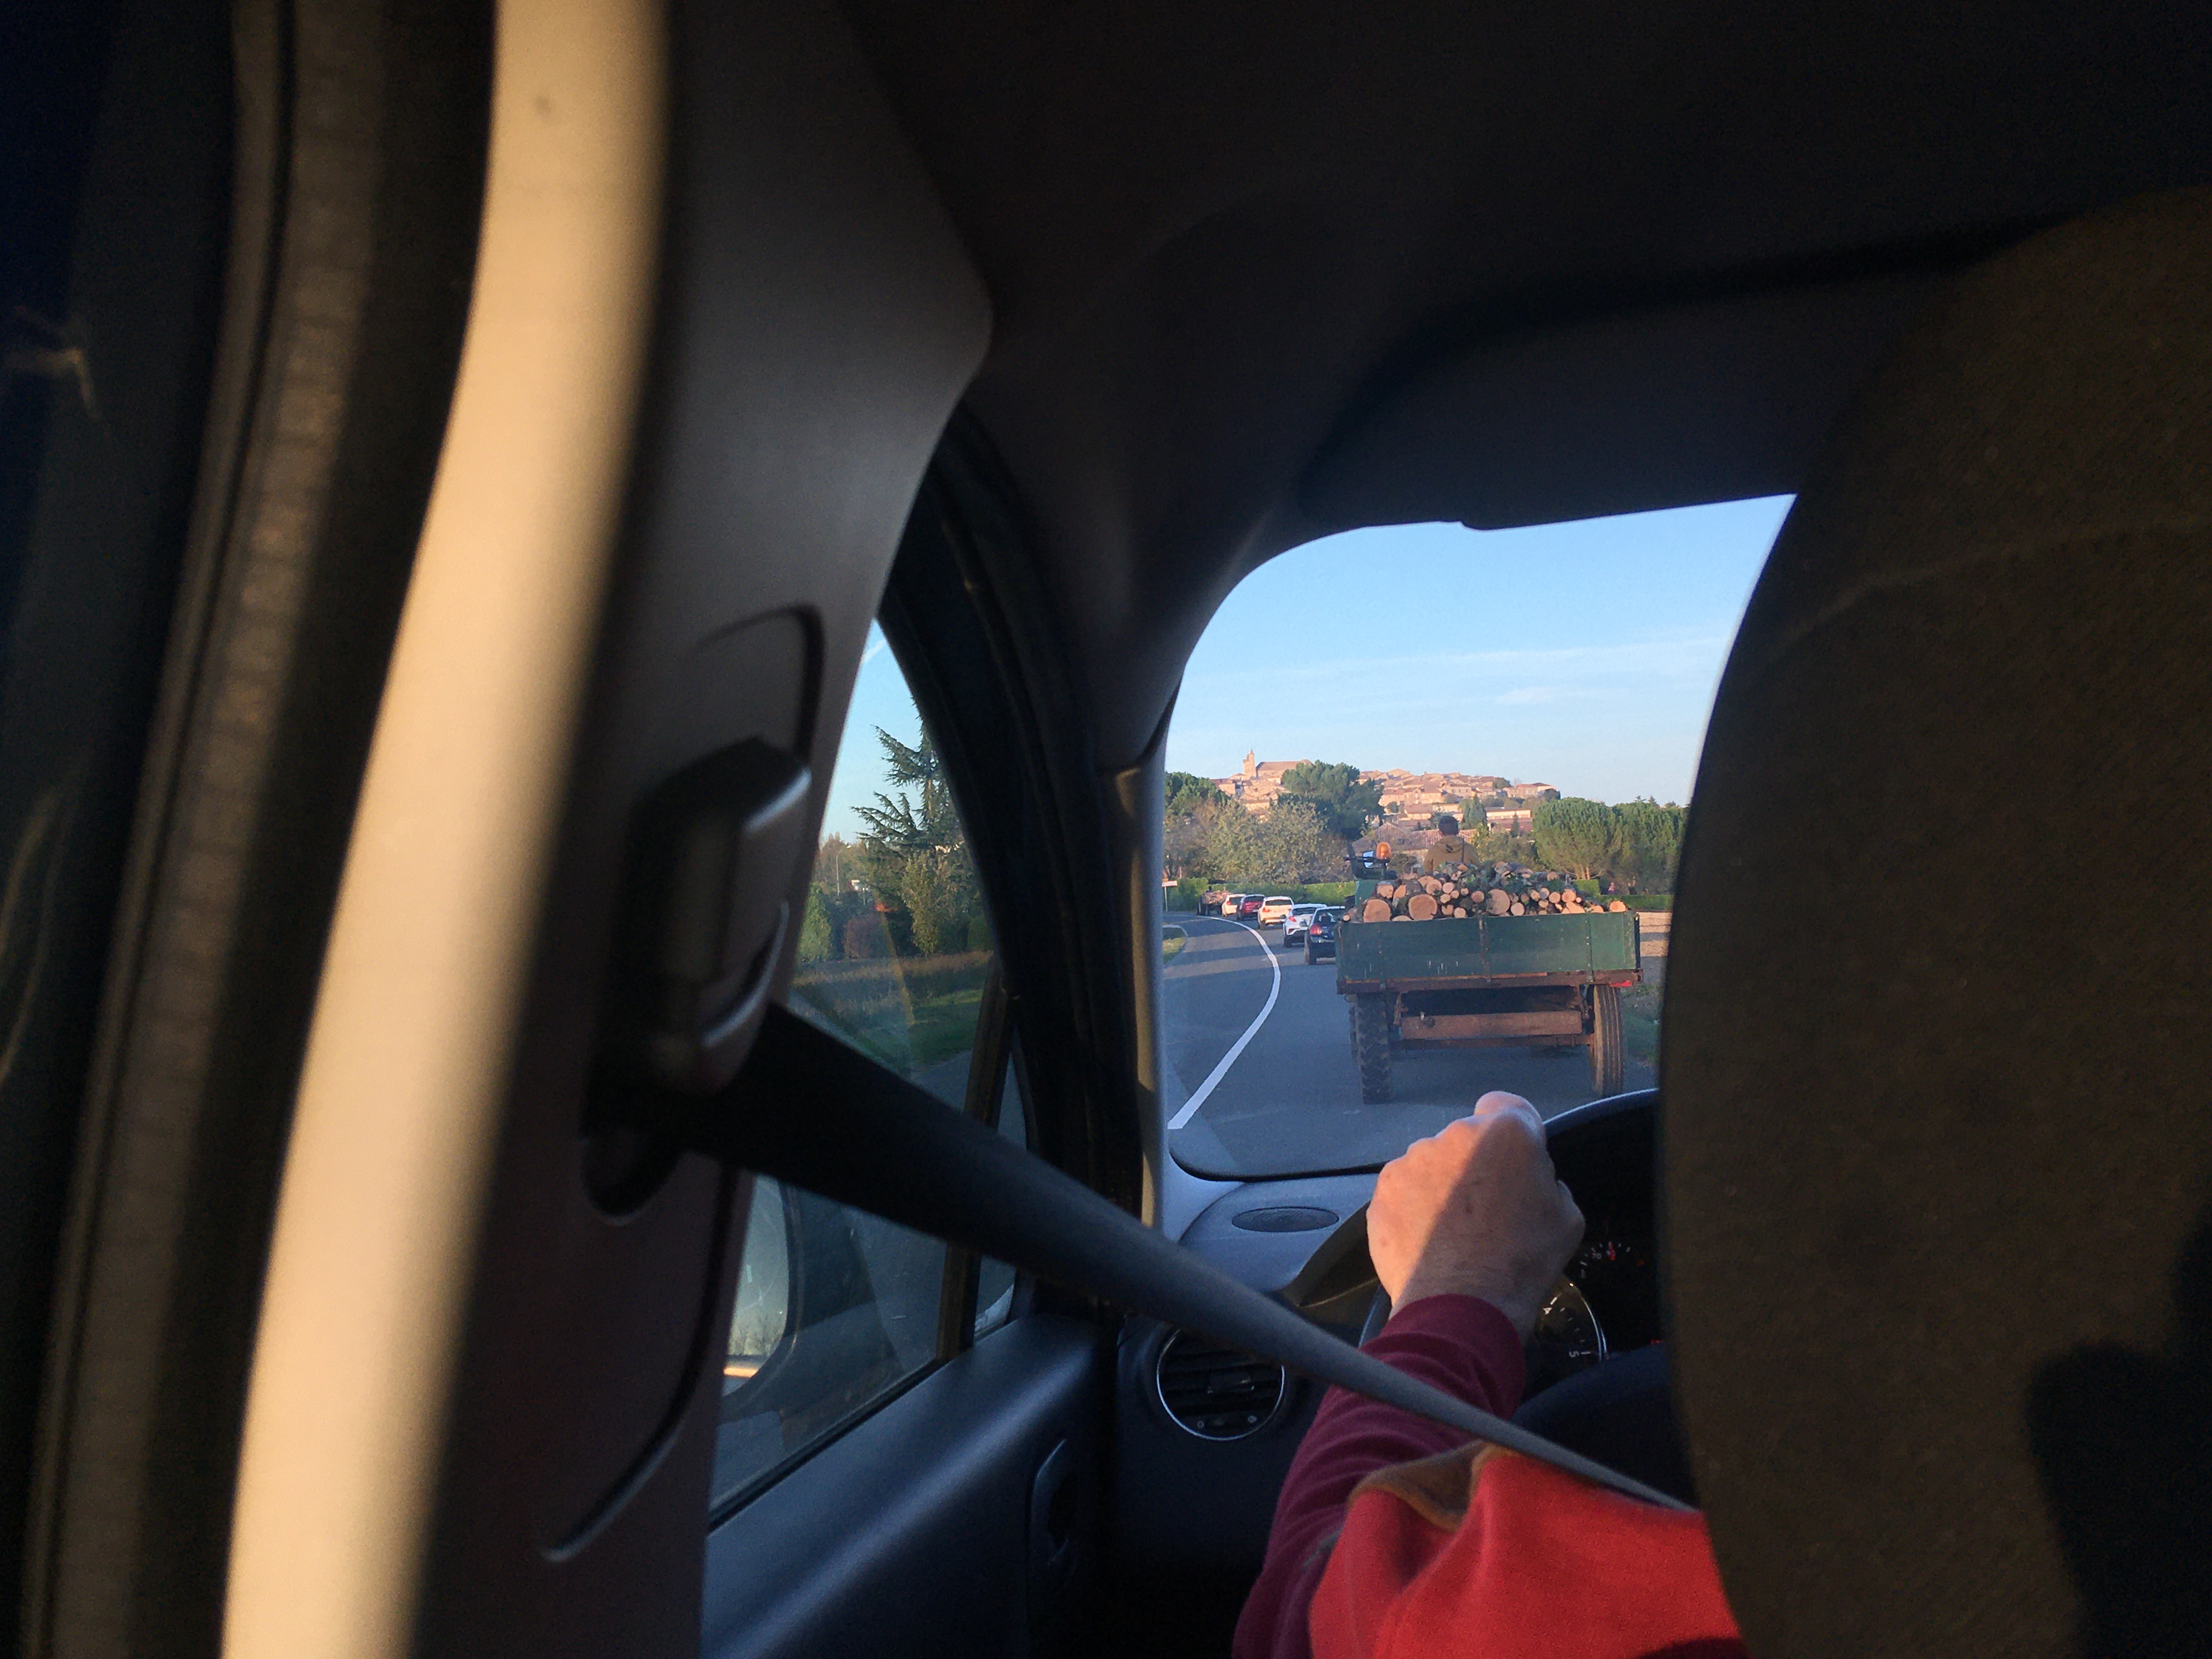
\includegraphics[width=\linewidth]{321}
		\caption{Patrick nous emmène dans un village vieux de 1000 ans.}
		\label{fig:image3}
	\end{minipage}
	\label{fig:myfigure}
\end{figure}

\begin{figure}[htbp]
	\centering
	\begin{minipage}{0.3\textwidth}
		\centering
		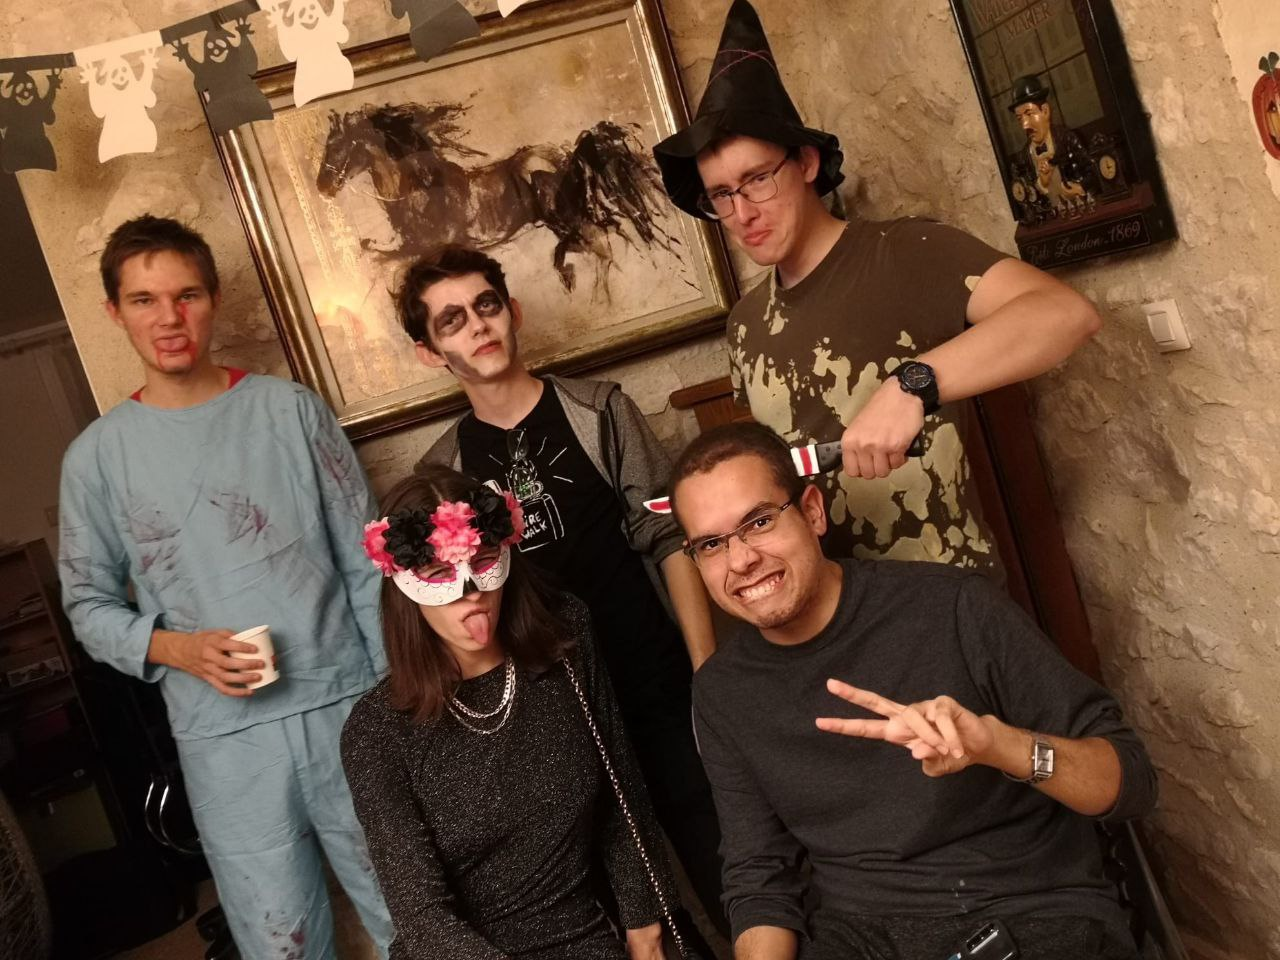
\includegraphics[width=\linewidth]{4}
		\caption{À l'occasion de Halloween dans la famille d'accueil de mon ami}
		\label{fig:image1}
	\end{minipage}
	\hfill
	\begin{minipage}{0.3\textwidth}
		\centering
		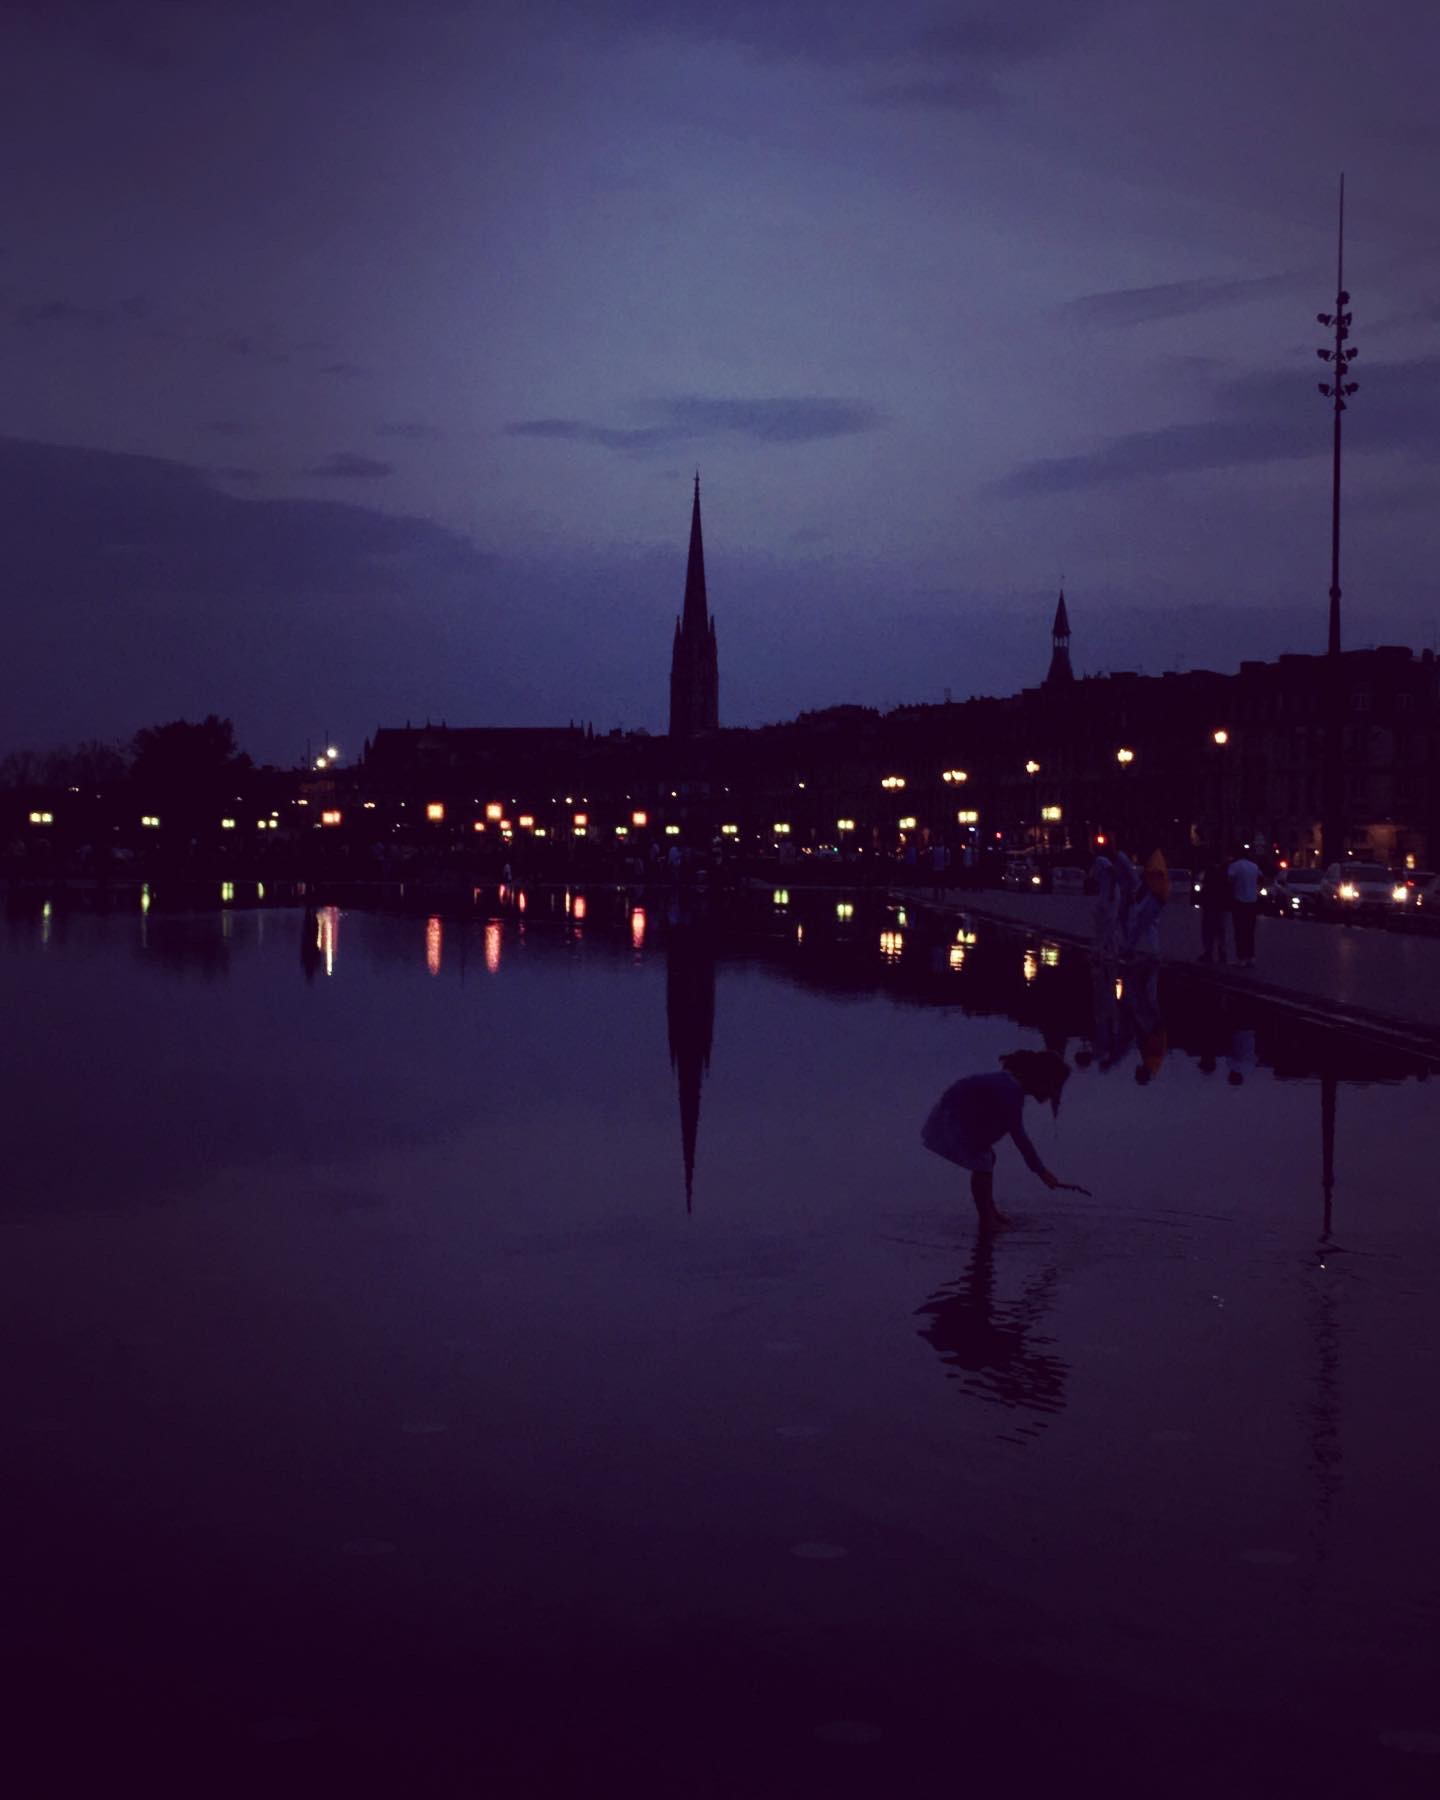
\includegraphics[width=\linewidth]{43}
		\caption{La photo prise à Bordeaux lors d'un week-end à Villeneuve}
		\label{fig:image2}
	\end{minipage}
	\hfill
	\begin{minipage}{0.3\textwidth}
		\centering
		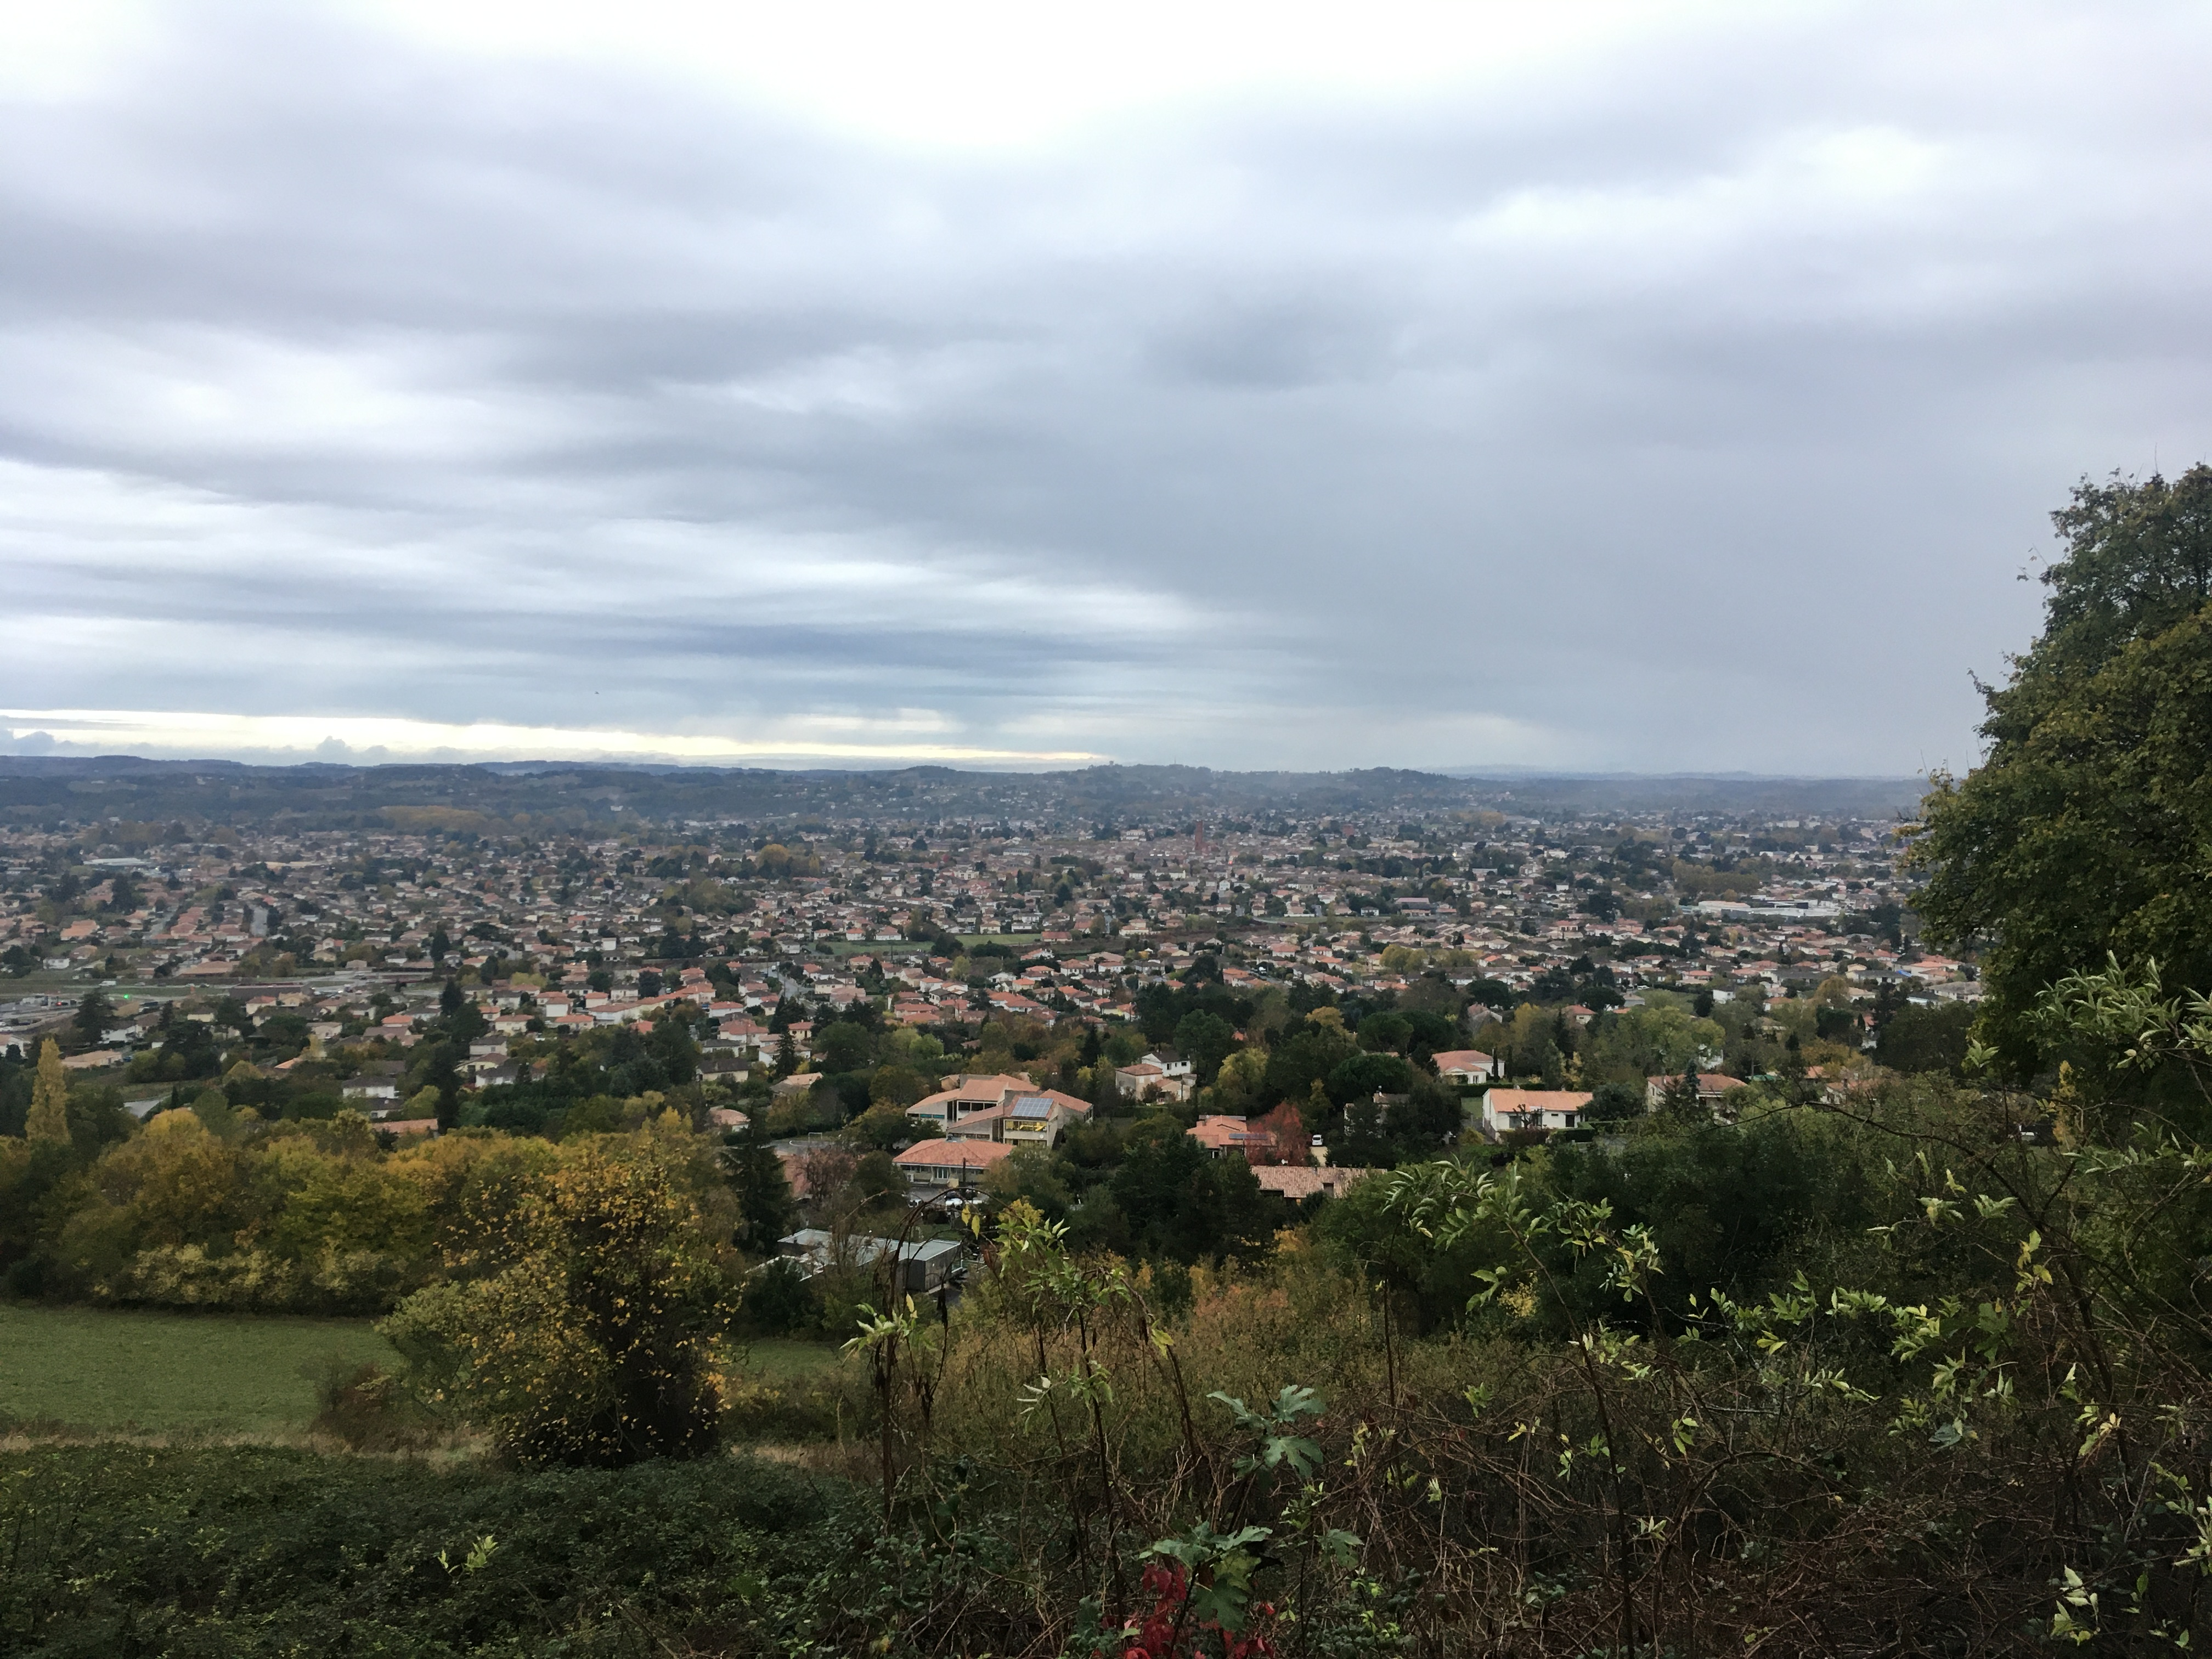
\includegraphics[width=\linewidth]{123}
		\caption{Une photo de Villeneuve que j'ai prise lors de ma promenade}
		\label{fig:image3}
	\end{minipage}
	\label{fig:myfigure}
\end{figure}

\end{document}